%!TEX program = xelatex
\documentclass[UTF8]{ctexart}
    \usepackage{amsmath}
    \usepackage{geometry}
	\usepackage{graphicx}
	\usepackage[utf8]{inputenc}
	\usepackage{listings}
	\usepackage{url}
	\usepackage{verbatim}
	
	\graphicspath{ {./images/} }

    \title{词法分析程序说明文档}
    \author{2016211305班 \ 熊光正 (学号:2016211249)}
    \date{\today}
\begin{document}
\lstset{numbers=left,frame=single}
\maketitle
\tableofcontents
\clearpage
\section{符号说明}
\begin{enumerate}
	\item $[a-bc-de...]$: 序列中$a$至$b$、$c$至$d$或$e$中的任意字符;
	\item $[\wedge a-bc-de...]$: 不在序列中$a$至$b$、$c$至$d$或$e$中的任意字符;
	\item $languages$: 所有合法字符串;
	\item $ints$: 一个无符号整数;
	\item $octs$: 8进制无符号整数;
	\item $oct = [0-7]$: 0 至 7 的一位阿拉伯数字;
	\item $decs$: 10进制无符号整数;
	\item $dec = [0-9]$: 0 至 9 的一位阿拉伯数字;
	\item $dec1 = [1-9]$: 1 至 9 的一位阿拉伯数字;
	\item $hexs$: 16进制无符号整数;
	\item $hex = [1-9a-eA-E]$: 0 至 9 的一位阿拉伯数字,或$A$至$E$的一位大小写字母;
	\item $floats$: 10进制无符号浮点数;
	\item $float_no_e$: 10进制无符号、没有使用科学记数法表示的浮点数;
	\item $chars$: 字符型;
	\item $char$: 一位任意字符;
	\item $charNoSqBs = [\wedge '\backslash]$: 一位非单引号、也非反斜线(转义符)的字符;
	\item $charInString = [\wedge "]$: 一位非双引号的字符;
	\item $charNoBl = [\wedge \backslash n]$: 一位非换行符的字符,可出现在单行注释中;
	\item $charNoStar = [\wedge *]$: 一位非星号的字符,用于跨行注释的识别;
	\item $charNoBs = [\wedge /]$: 一位非反斜杠的字符,用于跨行注释的识别;
	\item $letter$: 考虑到一位大小写字母字符的功能与下划线相等,我们用$letter$表示一位大小写字母字符或下划线;
	\item $strings$: 字符串型;
	\item $keyword$: 关键字;
	\item $identifier$: 标识符;
\end{enumerate}
注:为便于识别,必要时,我们使用空格分隔正则表达式中的各个符号。
\section{文法的推导与设计}
\subsection{关键字和标识符}
考虑到关键字和标识符均服从正则表达式$letter (letter|ddec|\_)^*$,我们先将其视为同一类型的符号,识别出再进行分类
,其文法为:
$$ identifier \rightarrow letter \ identifier1 $$
$$ identifier1 \rightarrow \varepsilon | letter \ identifier1 | dec \ identifier1 $$
\subsection{整数}
我们分别识别$8$进制、$10$进制和$16$进制的整数
\subsubsection{$8$进制整数}
以$0$开始,由$0$至$7$的整数组成,且长度不小于$2$,即
$$ octs = 0 \ {oct}^+ $$
,其文法为
$$ octs \rightarrow 0 \ octs1 $$
$$ octs1 \rightarrow oct \ octs2 $$
$$ octs2 \rightarrow \varepsilon | oct \ octs2 $$
\subsubsection{$10$进制整数}
若不以科学记数法表示,以$dec1$开始,由$dec$组成;若以科学记数法表示,则在不以科学记数法表示的整数的基础上
附加大小写英语字母$e$,正负号,和任意数字,即加上$0|((E|e)(+|-)?dec+)$。综上所述,其正则式为
$$ decs = 0 | dec1 \ dec+((E|e)(+|-)?dec+)? $$
其文法为
$$ decs \rightarrow dec1 \ decs1  $$
$$ decs1 \rightarrow \varepsilon | dec \ decs1 | E \ decs2 | e \ decs2 $$
$$ decs2 \rightarrow + \ decs3 | - \ decs3 | dec \ decs4  $$
$$ decs3 \rightarrow dec \ decs4  $$
$$ decs4 \rightarrow \varepsilon | dec \ decs4  $$
\subsubsection{$16$进制整数}
以$0x$开始,由$hex$组成,且长度不小于$3$,即
$$ hexs = 0 \ x  \ {hex}^+ $$
其文法为
$$ hexs \rightarrow 0 \ hexs1 $$
$$ hexs1 \rightarrow x \ hexs2 $$
$$ hexs2 \rightarrow hex \ hexs3 $$
$$ hexs3 \rightarrow \varepsilon | hex \ hexs3 $$
\subsubsection{所有整数}
综上所述,整数的文法为
$$ ints \rightarrow 0 \ octs1hexs1dec0 | dec1 \ decs1 $$
$$ octs1hexs1dec0 \rightarrow \varepsilon | oct \ octs2 | x \ hexs2 $$
$$ octs2 \rightarrow \varepsilon | oct \ octs2 $$
$$ hexs2 \rightarrow hex \ hexs3 $$
$$ hexs3 \rightarrow \varepsilon | hex \ hexs3 $$
$$ decs1 \rightarrow \varepsilon | dec \ decs1 | E \ decs2 | e \ decs2 $$
$$ decs2 \rightarrow + \ decs3 | - \ decs3 | dec \ decs4  $$
$$ decs3 \rightarrow dec \ decs4  $$
$$ decs4 \rightarrow \varepsilon | dec \ decs4  $$
依据上述文法识别到整型后,我们通过$atoi$函数将其转换为整数。
\subsection{浮点数}
对于非科学记数法表示的浮点数,其小数点前、后的部分可分别视为一个$10$进制整数;对于科学记数法表示的浮点数,
其指数部分可以视为一个$10$进制有符号或无符号整数。故其正则式为
$$ floats = decs.{dec}^+(e|E)(+|-)dec $$
,其文法为
$$ floats \rightarrow dec1 \ floats1 $$
$$ floats1 \rightarrow dec \ floats1 | . \ floats2 $$
$$ floats2 \rightarrow dec \ floats3 $$
$$ floats3 \rightarrow \varepsilon | dec \ floats3 | e \ floats4 | E \ floats4 $$
$$ floats4 \rightarrow + \ floats5 | - \ floats5 | dec \ floats6 $$
$$ floats5 \rightarrow dec \ floats6 $$
$$ floats6 \rightarrow \varepsilon | dec \ floats6 $$
依据上述文法识别到浮点型后,我们通过$atof$函数将其转换为浮点数
\subsection{(单个)字符}
由单引号、非单引号字符、单引号组成,其正则式为
$$ ` \ (charNoSqBs | \backslash \ char) \ ' $$
,其文法为
$$ chars \rightarrow ' \ chars1 $$
$$ chars1 \rightarrow \backslash \ chars2 | charNoSqBs \ chars3 $$
$$ chars2 \rightarrow char \ chars3 $$
$$ chars3 \rightarrow ' $$
\subsection{字符串}
由双引号、非双引号也非换行符的字符、双引号组成,其正则式为
$$ '' \ {(charInString | \backslash \ char)}^* \ '' $$
,其文法为
$$ strings \rightarrow '' \ strings1 $$
$$ strings1 \rightarrow '' | \backslash strings2 | charInString \ strings1 $$
$$ strings2 \rightarrow char \ strings1 $$
\subsection{运算符}
我们借用语法分析中的首符号集的概念,对各个运算符进行分析,得到如下文法
\begin{equation}
	\begin{aligned}
		UnaryOperators \rightarrow & . | ? | \sim | - \ Operators1 | ! \ Operators2 | \% \ Operators3 | \& \ Operators4 \\
		                           & | * \ Operators5 | / | Operators6 | \wedge \ Operators7 | \ | \ Operators8         \\
		                           & | + \ Operators9 | < \ Operators10 | = \ Operators11 | > \ Operators12             \\
		                           & | \colon \ Operators15
	\end{aligned}
\end{equation}
$$ Operators1 \rightarrow \varepsilon | - | = $$
$$ Operators2 \rightarrow \varepsilon | = $$
$$ Operators3 \rightarrow \varepsilon | = $$
$$ Operators4 \rightarrow \varepsilon | \& | = $$
$$ Operators5 \rightarrow \varepsilon | = $$
$$ Operators6 \rightarrow \varepsilon | = $$
$$ Operators7 \rightarrow \varepsilon | = $$
$$ Operators8 \rightarrow \varepsilon | \ | | \ = $$
$$ Operators9 \rightarrow \varepsilon | + | = $$
$$ Operators10 \rightarrow \varepsilon | = | < Operators13 $$
$$ Operators11 \rightarrow \varepsilon | = $$
$$ Operators12 \rightarrow \varepsilon | = | > Operators14 $$
$$ Operators13 \rightarrow \varepsilon | = $$
$$ Operators14 \rightarrow \varepsilon | = $$
$$ Operators15 \rightarrow \varepsilon | \colon $$
\subsection{界符}
分析可知每个界符(终结符)均仅在一个非终结符的首符号集中,故凡遇到终结符界符,即可认定遇到了界符符号,其文法为
$$ delimiters \rightarrow (  \ | \  )  \ | \  [  \ | \  ]  \ | \  \{  \ | \  \}  \ | \  ,  \ | \  ; $$
\subsection{注释}
\subsubsection{单行注释}
由$//$开始,遇到换行符,其正则式为
$$ / \ / \ {charNoBl}^* \ \backslash n $$
,其文法为
$$ commentInLine \rightarrow / \ commentInLine1 $$
$$ commentInLine1 \rightarrow / \ commentInLine2 $$
$$ commentInLine2 \rightarrow \backslash n | charNoBl \ commentInLine2 $$
\subsubsection{跨行注释}
由$/*$开始,遇到$*/$结束,其正则式为
$$ /*({charNoStar}^*|*{charNoBs})^**/ $$
,其文法为
$$ commentCrossLine \rightarrow / \ commentCrossLine1 $$
$$ commentCrossLine1 \rightarrow * \ commentCrossLine2 $$
$$ commentCrossLine2 \rightarrow * \ commentCrossLine3 | charNoStar \ commentCrossLine2 $$
$$ commentCrossLine3 \rightarrow / | charNoBs \ commentCrossLine2 $$
\subsubsection{宏}
为简化程序,我们将以$\#$开始的宏也视为注释处理,其正则式为
$$ \# {charNoBl}^* \ \backslash n $$
,其文法为
$$ commentOfMacros \rightarrow \# \ commentOfMacros1 $$
$$ commentOfMacros1 \rightarrow \backslash n | charNoBl \ commentOfMacros1 $$
\subsubsection{所有注释}
综上所述,注释的文法为
$$ comments \rightarrow / \ comments1 | \# \ commentOfMacros1 $$
$$ comments1 \rightarrow / \ commentInLine2 |* \ commentCrossLine2  $$
$$ commentInLine2 \rightarrow \backslash n | charNoBl \ commentInLine2 $$
$$ commentCrossLine2 \rightarrow * \ commentCrossLine3 | charNoStar \ commentCrossLine2 $$
$$ commentCrossLine3 \rightarrow / | charNoBs \ commentCrossLine2 $$
$$ commentOfMacros1 \rightarrow \backslash n | charNoBl \ commentOfMacros1 $$
\subsection{所有文法}
\begin{equation}
	\begin{aligned}
		languages & \rightarrow 0 \ octs1hexs1dec0 | dec1 \ decs1floats1 | ' \ chars1 | '' \ strings1                                   \\
		          & | - \ Operators1 | ! \ Operators2 | \% \ Operators3  | \& \ Operators4                                              \\
		          & | * \ Operators5  | / \ Operators6comments1 | \wedge \ Operators7                                                   \\
		          & | \ | \ Operators8 | + \ Operators9  | < \ Operators10 | = \ Operators11                                            \\
		          & | > \ Operators12  | \colon \ Operators15 | letter \ identifier1                                                    \\
		          & | \# \ commentOfMacros1  | . | ? | \sim | (  \ | \  )  \ | \  [  \ | \  ]  \ | \  \{  \ | \  \}  \ | \  ,  \ | \  ;
	\end{aligned}
\end{equation}
\begin{equation}
	identifier1 \rightarrow \varepsilon | letter \ identifier1 | dec \ identifier1
\end{equation}
\begin{equation}
	octs1hexs1dec0 \rightarrow \varepsilon | . \ floats2 | oct \ octs2 | x \ hexs2
\end{equation}
\begin{equation}
	octs2 \rightarrow \varepsilon | . \ floats2 | oct \ octs2
\end{equation}
\begin{equation}
	hexs2 \rightarrow hex \ hexs3
\end{equation}
\begin{equation}
	hexs3 \rightarrow \varepsilon | hex \ hexs3
\end{equation}
\begin{equation}
	decs1floats1 \rightarrow \varepsilon | dec \ decs1floats1 | E \ decs2 | e \ decs2 | . \ floats2
\end{equation}
\begin{equation}
	decs2 \rightarrow + \ decs3 | - \ decs3 | dec \ decs4
\end{equation}
\begin{equation}
	decs3 \rightarrow dec \ decs4
\end{equation}
\begin{equation}
	decs4 \rightarrow \varepsilon | dec \ decs4
\end{equation}
\begin{equation}
	floats2 \rightarrow dec \ floats3
\end{equation}
\begin{equation}
	floats3 \rightarrow \varepsilon | dec \ floats3 | e \ floats4 | E \ floats4
\end{equation}
\begin{equation}
	floats4 \rightarrow + \ floats5 | - \ floats5 | dec \ floats6
\end{equation}
\begin{equation}
	floats5 \rightarrow dec \ floats6
\end{equation}
\begin{equation}
	floats6 \rightarrow \varepsilon | dec \ floats6
\end{equation}
\begin{equation}
	chars1 \rightarrow \backslash \ chars2 | charNoSqBs \ chars3
\end{equation}
\begin{equation}
	chars2 \rightarrow char \ chars3
\end{equation}
\begin{equation}
	chars3 \rightarrow '
\end{equation}
\begin{equation}
	strings1 \rightarrow '' | \backslash strings2 | charInString \ strings1
\end{equation}
\begin{equation}
	strings2 \rightarrow char \ strings1
\end{equation}
\begin{equation}
	\begin{aligned}
		Operators6comments1 \rightarrow \varepsilon | = & | / \ commentInLine2   \\
		                                                & |* \ commentCrossLine2
	\end{aligned}
\end{equation}
\begin{equation}
	commentInLine2 \rightarrow \backslash n | charNoBl \ commentInLine2
\end{equation}
\begin{equation}
	\begin{aligned}
		commentCrossLine2 \rightarrow & * \ commentCrossLine3            \\
		                              & | charNoStar \ commentCrossLine2
	\end{aligned}
\end{equation}
\begin{equation}
	commentCrossLine3 \rightarrow / | charNoBs \ commentCrossLine2
\end{equation}
\begin{equation}
	commentOfMacros1 \rightarrow \backslash n | charNoBl \ commentOfMacros1
\end{equation}
\begin{equation}
	Operators1 \rightarrow \varepsilon | - | =
\end{equation}
\begin{equation}
	Operators2 \rightarrow \varepsilon | =
\end{equation}
\begin{equation}
	Operators3 \rightarrow \varepsilon | =
\end{equation}
\begin{equation}
	Operators4 \rightarrow \varepsilon | \& | =
\end{equation}
\begin{equation}
	Operators5 \rightarrow \varepsilon | =
\end{equation}
\begin{equation}
	Operators7 \rightarrow \varepsilon | =
\end{equation}
\begin{equation}
	Operators8 \rightarrow \varepsilon | \ | | \ =
\end{equation}
\begin{equation}
	Operators9 \rightarrow \varepsilon | + | =
\end{equation}
\begin{equation}
	Operators10 \rightarrow \varepsilon | = | < Operators13
\end{equation}
\begin{equation}
	Operators11 \rightarrow \varepsilon | =
\end{equation}
\begin{equation}
	Operators12 \rightarrow \varepsilon | = | > Operators14
\end{equation}
\begin{equation}
	Operators13 \rightarrow \varepsilon | =
\end{equation}
\begin{equation}
	Operators14 \rightarrow \varepsilon | =
\end{equation}
\begin{equation}
	Operators15 \rightarrow \varepsilon | \colon
\end{equation}
\section{开发环境}
本程序使用$Visual \ Studio \ Code$编辑器,在基于$x86_64$指令集的$64$位中文$Windows \ 10$环境下开发。
程序使用$Clang++$(版本号:$7.0.0$)编译器,基于$c++14$标准和$MSVC$环境进行静态编译。
\section{运行环境}
本程序支持在$64$位中文$Windows \ 10$环境下运行,没有其他运行时依赖。
\section{功能实现}
程序定义了$TokenValueUnion$类以记录符号的数据,定义了$TokenType$枚举以表述符号的类型,
并使用$std::pair<TokenType, TokenValueUnion>$表示符号的类型和对应的数据。
程序定义了$TextReader$类以建立、管理缓冲区,统计相关信息,并抽象化文件的读取。
程序使用$std::unordered_map$定义了关键字、运算符和界符,并构建了符号表。
程序定义了$Lexer$类以完成词法分析的功能,其中,$void Lexer::prase(const string \&filename)$函数执行从文件中分析词法的功能。
依据前文推到的文法,该函数中的自动机依次比对各个字符以识别符号,并处理错误。
\section{程序功能}
\subsection{识别合法符号及注释}
依据上述文本,本程序可以识别科学记数法或非科学记数法表示的$8$、$10$、$16$进制的无符号整数和浮点数、带转义或不带转义的单个字符或字符串
,各类括号或分号等界符,以及文法中列举的各类操作符。词法分析程序会识别并跳过行内和跨行注释,和$\#$开始的宏指令。
\subsection{统计文本信息}
本程序可以统计并输出源文件的行数和字符总数。
\subsection{错误处理}
本程序可以识别源文件中出现的词法错误,报告其所在行数、列数,并继续分析后面的源代码。对于字符型中缺失后单引号,词法处理程序可以自动纠正。
\section{运行流程}
根据需求分批读取字符至缓冲区,依次分析并形成符号串,对标识符建立符号表,同时统计行数、字符串、符号数和错误数。
若出现自动机无法识别的字符,尝试进行纠正并继续运行至文件尾。
\section{使用说明}
运行程序后根据提示输入目标文件名,或将目标文件拖拽至词法分析程序的可执行文件上。
\section{样例使用说明}
\subsection{合法源文件样例}
\subsubsection{基础测试样例:$legal\_1.cpp$}
本样例测试标识符、科学记数法或非科学记数法表示的$10$进制整数、浮点数、基本运算符和界符的识别及注释的处理等基本要求,源代码中不含词法错误。
\begin{lstlisting}[language={C++}]
/*
    基础测试样例
*/

int main(int argc, char const *argv[])
{
    const int _a_1 = 0, B__c__2 = 11E4;
    double d25sd5r6tf7gy890jn = 0.3e-2;
    float d = -0.01;
    d25sd5r6tf7gy890jn -= (_a_1 - B__c__2 * (d / _a_1));
    d += (_a_1 % B__c__2);
    return --d;
}
\end{lstlisting}
将$legal\_1.cpp$文件拖拽至$main.exe$文件上,分析输出 \\
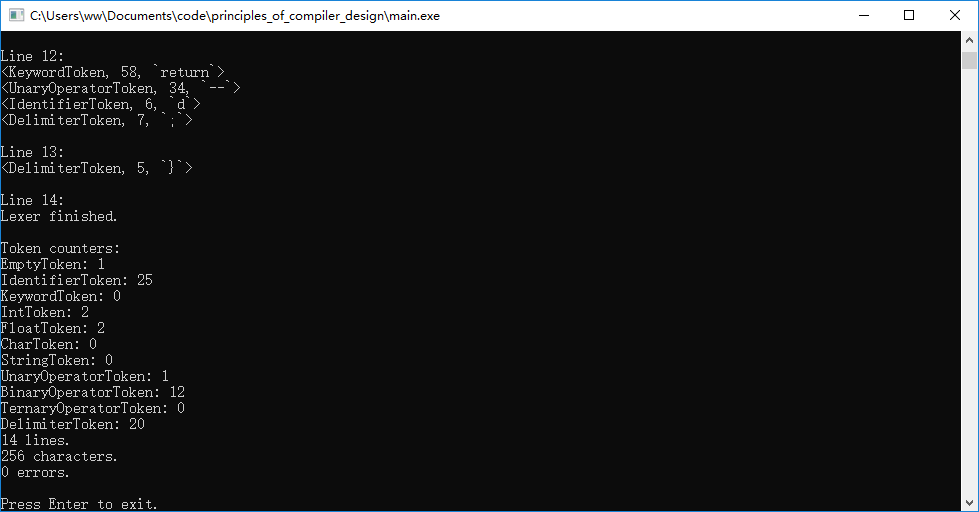
\includegraphics[width=\textwidth]{legal_1}
\begin{lstlisting}
Line 1

Line 2:

Line 3:
<EmptyToken, 1, `*
    基础测试样例
*`>

Line 4:

Line 5:
<KeywordToken, 40, `int`>
<IdentifierToken, 0, `main`>
<DelimiterToken, 0, `(`>
<KeywordToken, 40, `int`>
<IdentifierToken, 1, `argc`>
<DelimiterToken, 6, `,`>
<KeywordToken, 12, `char`>
<KeywordToken, 18, `const`>
<BinaryOperatorToken, 9, `*`>
<IdentifierToken, 2, `argv`>
<DelimiterToken, 2, `[`>
<DelimiterToken, 3, `]`>
<DelimiterToken, 1, `)`>

Line 6:
<DelimiterToken, 4, `{`>

Line 7:
<KeywordToken, 18, `const`>
<KeywordToken, 40, `int`>
<IdentifierToken, 3, `_a_1`>
<BinaryOperatorToken, 14, `=`>
<IntToken, 0, `0`>
<DelimiterToken, 6, `,`>
<IdentifierToken, 4, `B__c__2`>
<BinaryOperatorToken, 14, `=`>
<IntToken, 11, `11E4`>
<DelimiterToken, 7, `;`>

Line 8:
<KeywordToken, 26, `double`>
<IdentifierToken, 5, `d25sd5r6tf7gy890jn`>
<BinaryOperatorToken, 14, `=`>
<FloatToken, 0.003000, `0.3e-2`>
<DelimiterToken, 7, `;`>

Line 9:
<KeywordToken, 34, `float`>
<IdentifierToken, 6, `d`>
<BinaryOperatorToken, 14, `=`>
<BinaryOperatorToken, 8, `-`>
<FloatToken, 0.010000, `0.01`>
<DelimiterToken, 7, `;`>

Line 10:
<IdentifierToken, 5, `d25sd5r6tf7gy890jn`>
<BinaryOperatorToken, 18, `-=`>
<DelimiterToken, 0, `(`>
<IdentifierToken, 3, `_a_1`>
<BinaryOperatorToken, 8, `-`>
<IdentifierToken, 4, `B__c__2`>
<BinaryOperatorToken, 9, `*`>
<DelimiterToken, 0, `(`>
<IdentifierToken, 6, `d`>
<BinaryOperatorToken, 10, `/`>
<IdentifierToken, 3, `_a_1`>
<DelimiterToken, 1, `)`>
<DelimiterToken, 1, `)`>
<DelimiterToken, 7, `;`>

Line 11:
<IdentifierToken, 6, `d`>
<BinaryOperatorToken, 17, `+=`>
<DelimiterToken, 0, `(`>
<IdentifierToken, 3, `_a_1`>
<BinaryOperatorToken, 13, `%`>
<IdentifierToken, 4, `B__c__2`>
<DelimiterToken, 1, `)`>
<DelimiterToken, 7, `;`>

Line 12:
<KeywordToken, 58, `return`>
<UnaryOperatorToken, 34, `--`>
<IdentifierToken, 6, `d`>
<DelimiterToken, 7, `;`>

Line 13:
<DelimiterToken, 5, `}`>

Line 14:
Lexer finished.

Token counters:
EmptyToken: 1
IdentifierToken: 25
KeywordToken: 0
IntToken: 2
FloatToken: 2
CharToken: 0
StringToken: 0
UnaryOperatorToken: 1
BinaryOperatorToken: 12
TernaryOperatorToken: 0
DelimiterToken: 20
14 lines.
256 characters.
0 errors.

Press Enter to exit.
\end{lstlisting}
词法分析程序分析出了所有合法的符号,包括标识符、科学记数法或非科学记数法表示的$10$进制整数、浮点数、基本运算符和界符,并得到了行数、符号数与错误数。

\subsubsection{延伸测试样例-多进制整数:$legal\_2.cpp$}
本样例测试$8$进制、$16$进制整数的识别等延伸特性,源代码中不含词法错误。
\begin{lstlisting}
/*
    延伸测试样例-多进制整数
*/

int main(int argc, char const *argv[])
{
    int a = 012, b = 0x12;
    const int c = 012e2, d = 0x12E3;
    a += 0x12E-3;
    a -= 012E-4;
    return 0;
}
\end{lstlisting}
将$legal\_2.cpp$文件拖拽至$main.exe$文件上,分析输出 \\
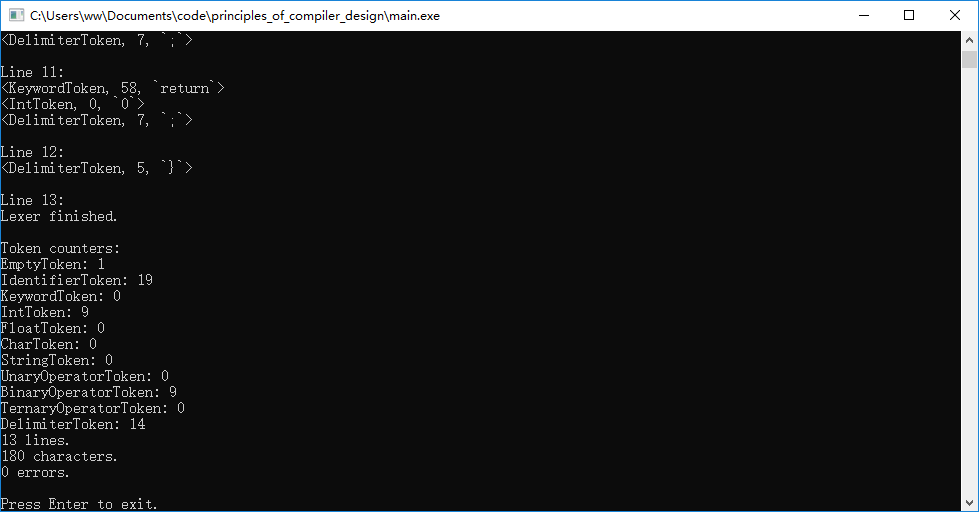
\includegraphics[width=\textwidth]{legal_2}
\begin{lstlisting}
Line 1

Line 2:

Line 3:
<EmptyToken, 1, `*
    延伸测试样例-多进制整数
*`>

Line 4:

Line 5:
<KeywordToken, 40, `int`>
<IdentifierToken, 0, `main`>
<DelimiterToken, 0, `(`>
<KeywordToken, 40, `int`>
<IdentifierToken, 1, `argc`>
<DelimiterToken, 6, `,`>
<KeywordToken, 12, `char`>
<KeywordToken, 18, `const`>
<BinaryOperatorToken, 9, `*`>
<IdentifierToken, 2, `argv`>
<DelimiterToken, 2, `[`>
<DelimiterToken, 3, `]`>
<DelimiterToken, 1, `)`>

Line 6:
<DelimiterToken, 4, `{`>

Line 7:
<KeywordToken, 40, `int`>
<IdentifierToken, 3, `a`>
<BinaryOperatorToken, 14, `=`>
<IntToken, 12, `012`>
<DelimiterToken, 6, `,`>
<IdentifierToken, 4, `b`>
<BinaryOperatorToken, 14, `=`>
<IntToken, 0, `0x12`>
<DelimiterToken, 7, `;`>

Line 8:
<KeywordToken, 18, `const`>
<KeywordToken, 40, `int`>
<IdentifierToken, 5, `c`>
<BinaryOperatorToken, 14, `=`>
<IntToken, 12, `012`>
<IdentifierToken, 6, `e2`>
<DelimiterToken, 6, `,`>
<IdentifierToken, 7, `d`>
<BinaryOperatorToken, 14, `=`>
<IntToken, 0, `0x12E3`>
<DelimiterToken, 7, `;`>

Line 9:
<IdentifierToken, 3, `a`>
<BinaryOperatorToken, 17, `+=`>
<IntToken, 0, `0x12E`>
<BinaryOperatorToken, 8, `-`>
<IntToken, 3, `3`>
<DelimiterToken, 7, `;`>

Line 10:
<IdentifierToken, 3, `a`>
<BinaryOperatorToken, 18, `-=`>
<IntToken, 12, `012`>
<IdentifierToken, 8, `E`>
<BinaryOperatorToken, 8, `-`>
<IntToken, 4, `4`>
<DelimiterToken, 7, `;`>

Line 11:
<KeywordToken, 58, `return`>
<IntToken, 0, `0`>
<DelimiterToken, 7, `;`>

Line 12:
<DelimiterToken, 5, `}`>

Line 13:
Lexer finished.

Token counters:
EmptyToken: 1
IdentifierToken: 19
KeywordToken: 0
IntToken: 9
FloatToken: 0
CharToken: 0
StringToken: 0
UnaryOperatorToken: 0
BinaryOperatorToken: 9
TernaryOperatorToken: 0
DelimiterToken: 14
13 lines.
180 characters.
0 errors.

Press Enter to exit.
\end{lstlisting}
程序完整无误地识别出了所有$8$进制、$16$进制整数,并输出了统计信息。
\subsubsection{延伸测试样例-字符和字符串:$legal\_3.cpp$}
本样例测试含转义字符和不含转义字符的字符和字符串的识别等延伸特性,源代码中不含词法错误。
\begin{lstlisting}
#include <string>

/*
    延伸测试样例-字符和字符串
*/

int main(int argc, char const *argv[])
{
    char a = '1', b = '\'';
    std::string s = "string value\n", ss = "67gi8gb_+@#$%s^&*(oimk";
    return 0;
}
\end{lstlisting}
将$legal\_3.cpp$文件拖拽至$main.exe$文件上,分析输出 \\
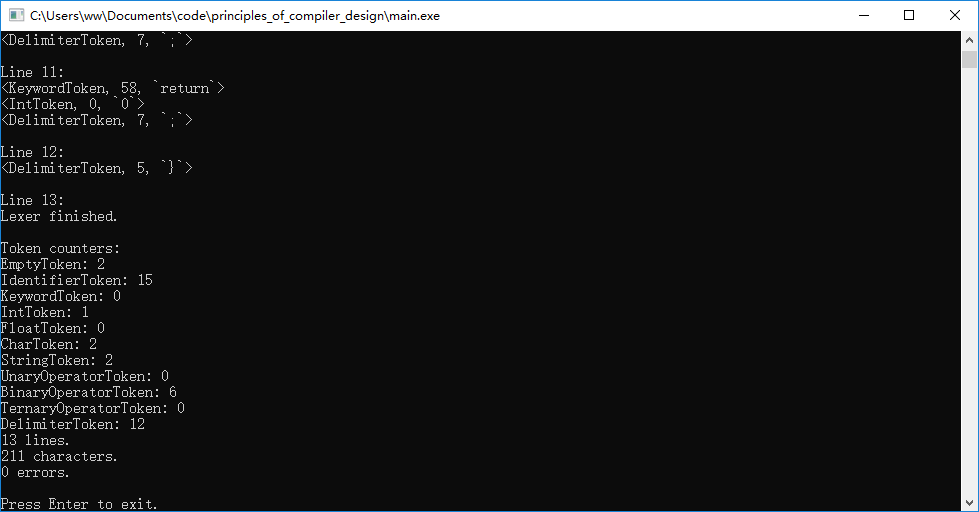
\includegraphics[width=\textwidth]{legal_3}
\begin{lstlisting}
Line 1
<EmptyToken, 1, `include <string`>

Line 2:

Line 3:

Line 4:

Line 5:
<EmptyToken, 1, `*
    寤朵几娴嬭瘯鏍蜂緥-瀛楃鍜屽瓧绗︿覆
*`>

Line 6:

Line 7:
<KeywordToken, 40, `int`>
<IdentifierToken, 0, `main`>
<DelimiterToken, 0, `(`>
<KeywordToken, 40, `int`>
<IdentifierToken, 1, `argc`>
<DelimiterToken, 6, `,`>
<KeywordToken, 12, `char`>
<KeywordToken, 18, `const`>
<BinaryOperatorToken, 9, `*`>
<IdentifierToken, 2, `argv`>
<DelimiterToken, 2, `[`>
<DelimiterToken, 3, `]`>
<DelimiterToken, 1, `)`>

Line 8:
<DelimiterToken, 4, `{`>

Line 9:
<KeywordToken, 12, `char`>
<IdentifierToken, 3, `a`>
<BinaryOperatorToken, 14, `=`>
<CharToken, 1, `1`>
<DelimiterToken, 6, `,`>
<IdentifierToken, 4, `b`>
<BinaryOperatorToken, 14, `=`>
<CharToken, \, `\'`>
<DelimiterToken, 7, `;`>

Line 10:
<IdentifierToken, 5, `std`>
<BinaryOperatorToken, 12, `::`>
<IdentifierToken, 6, `string`>
<IdentifierToken, 7, `s`>
<BinaryOperatorToken, 14, `=`>
<StringToken, `string value\n`>
<DelimiterToken, 6, `,`>
<IdentifierToken, 8, `ss`>
<BinaryOperatorToken, 14, `=`>
<StringToken, `67gi8gb_+@#$%s^&*(oimk`>
<DelimiterToken, 7, `;`>

Line 11:
<KeywordToken, 58, `return`>
<IntToken, 0, `0`>
<DelimiterToken, 7, `;`>

Line 12:
<DelimiterToken, 5, `}`>

Line 13:
Lexer finished.

Token counters:
EmptyToken: 2
IdentifierToken: 15
KeywordToken: 0
IntToken: 1
FloatToken: 0
CharToken: 2
StringToken: 2
UnaryOperatorToken: 0
BinaryOperatorToken: 6
TernaryOperatorToken: 0
DelimiterToken: 12
13 lines.
211 characters.
0 errors.

Press Enter to exit.
\end{lstlisting}
程序完整无误地识别出了所有含转义字符和不含转义字符的字符和字符串,并输出了统计信息。
\subsubsection{延伸测试样例-高级运算符及符号表:$legal\_4.cpp$}
本样例测试流操作等高级运算符的识别、符号表的建立和使用等延伸特性,源代码中不含词法错误。
\begin{lstlisting}
#include <iostream>
#include <string>

/*
    延伸测试样例-高级运算符及符号表
*/

class A
{
public:
    A();
    int s;
};

int main(int argc, char const *argv[])
{
    A aa;
    char a = '1', b = '\'';
    std::string s1 = "string value\n", s2 = "67gi8gb_+@#$%s^&*(oimk";
    std::cout << s1;
    std::cin >> s2;
    aa.s = (~2 | 4);
    a %= (&aa)->s;
    return 0;
}
\end{lstlisting}
将$legal\_4.cpp$文件拖拽至$main.exe$文件上,分析输出 \\
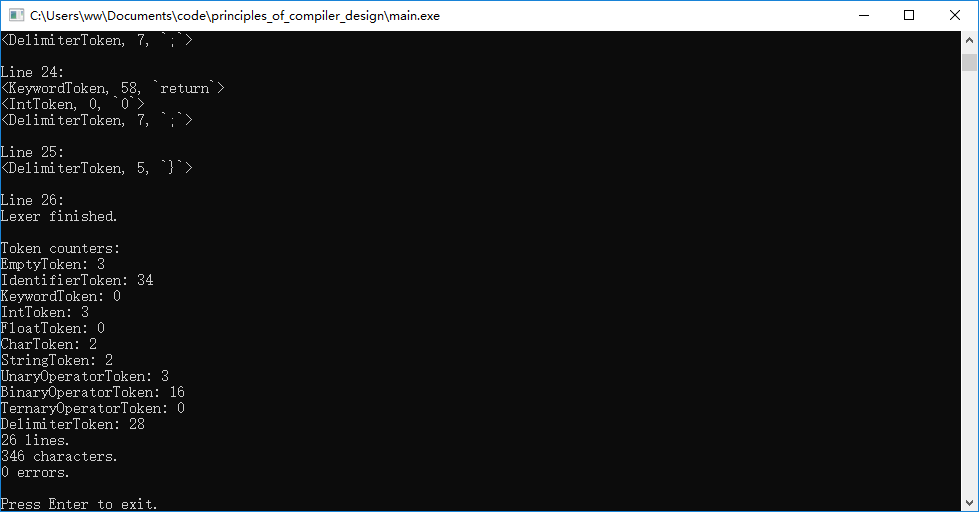
\includegraphics[width=\textwidth]{legal_4}
\begin{lstlisting}
Line 1
<EmptyToken, 1, `include <iostream`>

Line 2:
<EmptyToken, 1, `include <string`>

Line 3:

Line 4:

Line 5:

Line 6:
<EmptyToken, 1, `*
    延伸测试样例-高级运算符及符号表
*`>

Line 7:

Line 8:
<KeywordToken, 15, `class`>
<IdentifierToken, 0, `A`>

Line 9:
<DelimiterToken, 4, `{`>

Line 10:
<KeywordToken, 54, `public`>
<BinaryOperatorToken, 38, `:`>

Line 11:
<IdentifierToken, 0, `A`>
<DelimiterToken, 0, `(`>
<DelimiterToken, 1, `)`>
<DelimiterToken, 7, `;`>

Line 12:
<KeywordToken, 40, `int`>
<IdentifierToken, 1, `s`>
<DelimiterToken, 7, `;`>

Line 13:
<DelimiterToken, 5, `}`>
<DelimiterToken, 7, `;`>

Line 14:

Line 15:
<KeywordToken, 40, `int`>
<IdentifierToken, 2, `main`>
<DelimiterToken, 0, `(`>
<KeywordToken, 40, `int`>
<IdentifierToken, 3, `argc`>
<DelimiterToken, 6, `,`>
<KeywordToken, 12, `char`>
<KeywordToken, 18, `const`>
<BinaryOperatorToken, 9, `*`>
<IdentifierToken, 4, `argv`>
<DelimiterToken, 2, `[`>
<DelimiterToken, 3, `]`>
<DelimiterToken, 1, `)`>

Line 16:
<DelimiterToken, 4, `{`>

Line 17:
<IdentifierToken, 0, `A`>
<IdentifierToken, 5, `aa`>
<DelimiterToken, 7, `;`>

Line 18:
<KeywordToken, 12, `char`>
<IdentifierToken, 6, `a`>
<BinaryOperatorToken, 14, `=`>
<CharToken, 1, `1`>
<DelimiterToken, 6, `,`>
<IdentifierToken, 7, `b`>
<BinaryOperatorToken, 14, `=`>
<CharToken, \, `\'`>
<DelimiterToken, 7, `;`>

Line 19:
<IdentifierToken, 8, `std`>
<BinaryOperatorToken, 12, `::`>
<IdentifierToken, 9, `string`>
<IdentifierToken, 10, `s1`>
<BinaryOperatorToken, 14, `=`>
<StringToken, `string value\n`>
<DelimiterToken, 6, `,`>
<IdentifierToken, 11, `s2`>
<BinaryOperatorToken, 14, `=`>
<StringToken, `67gi8gb_+@#$%s^&*(oimk`>
<DelimiterToken, 7, `;`>

Line 20:
<IdentifierToken, 8, `std`>
<BinaryOperatorToken, 12, `::`>
<IdentifierToken, 12, `cout`>
<BinaryOperatorToken, 5, `<<`>
<IdentifierToken, 10, `s1`>
<DelimiterToken, 7, `;`>

Line 21:
<IdentifierToken, 8, `std`>
<BinaryOperatorToken, 12, `::`>
<IdentifierToken, 13, `cin`>
<BinaryOperatorToken, 6, `>>`>
<IdentifierToken, 11, `s2`>
<DelimiterToken, 7, `;`>

Line 22:
<IdentifierToken, 5, `aa`>
<BinaryOperatorToken, 11, `.`>
<IdentifierToken, 1, `s`>
<BinaryOperatorToken, 14, `=`>
<DelimiterToken, 0, `(`>
<UnaryOperatorToken, 3, `~`>
<IntToken, 2, `2`>
<UnaryOperatorToken, 2, `|`>
<IntToken, 4, `4`>
<DelimiterToken, 1, `)`>
<DelimiterToken, 7, `;`>

Line 23:
<IdentifierToken, 6, `a`>
<BinaryOperatorToken, 21, `%=`>
<DelimiterToken, 0, `(`>
<UnaryOperatorToken, 1, `&`>
<IdentifierToken, 5, `aa`>
<DelimiterToken, 1, `)`>
<BinaryOperatorToken, 8, `-`>
<BinaryOperatorToken, 16, `>`>
<IdentifierToken, 1, `s`>
<DelimiterToken, 7, `;`>

Line 24:
<KeywordToken, 58, `return`>
<IntToken, 0, `0`>
<DelimiterToken, 7, `;`>

Line 25:
<DelimiterToken, 5, `}`>

Line 26:
Lexer finished.

Token counters:
EmptyToken: 3
IdentifierToken: 34
KeywordToken: 0
IntToken: 3
FloatToken: 0
CharToken: 2
StringToken: 2
UnaryOperatorToken: 3
BinaryOperatorToken: 16
TernaryOperatorToken: 0
DelimiterToken: 28
26 lines.
346 characters.
0 errors.

Press Enter to exit.
\end{lstlisting}
程序完整无误地识别出了所有高级运算符,根据建立的符号表识别出了出现过的符号,并输出了统计信息。
\subsubsection{延伸测试样例-大规模真实数据:$legal\_5.cpp$}
本样例测试程序对大规模、真实数据的识别,源代码中不含词法错误。
将$legal\_5.cpp$文件拖拽至$main.exe$文件上,分析输出了所有符号的信息,因样例和输出太长,此处略去。 \\
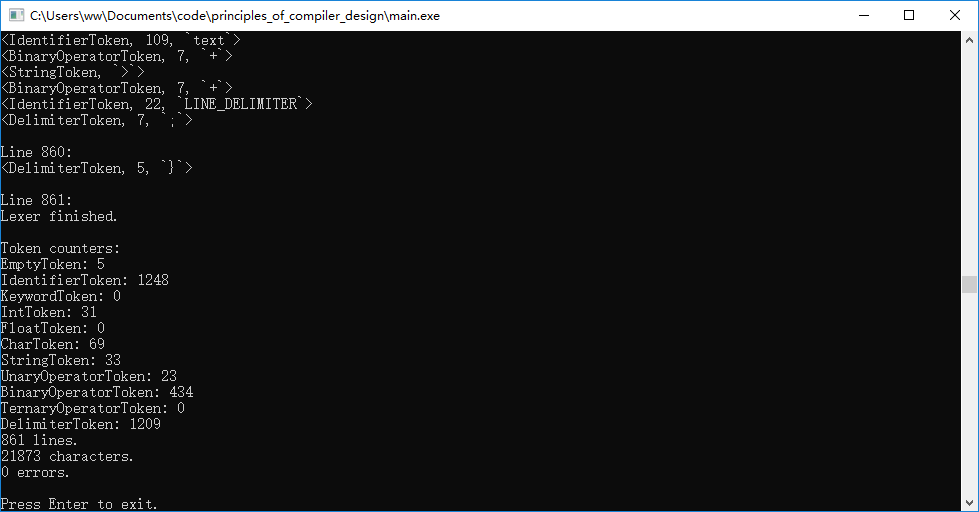
\includegraphics[width=\textwidth]{legal_5}
\subsection{含错误源文件样例}
\subsubsection{错误处理测试样例-常数中的错误:$illegal\_1.cpp$}
\begin{lstlisting}
/*
    错误处理测试样例-常数中的错误
*/

int main(int argc, char const *argv[])
{
    const int _a = ~0., B_ = 11;
    double d2 = 0.3e2 + _a;
    int j = 0xz1, k = 011;
    return 0;
}
\end{lstlisting}
将$illegal\_1.cpp$文件拖拽至$main.exe$文件上,分析输出 \\
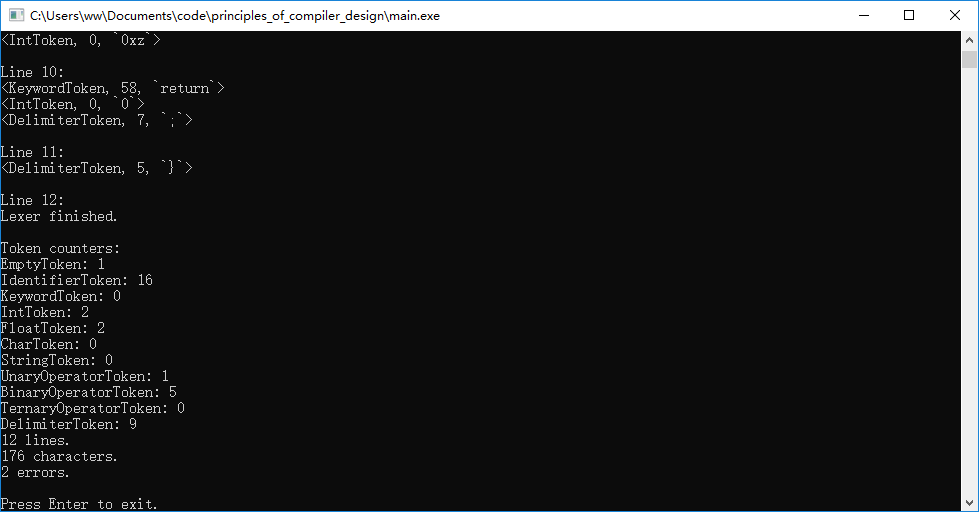
\includegraphics[width=\textwidth]{illegal_1}
\begin{lstlisting}
Line 1

Line 2:

Line 3:
<EmptyToken, 1, `*
    错误处理测试样例-常数中的错误
*`>

Line 4:

Line 5:
<KeywordToken, 40, `int`>
<IdentifierToken, 0, `main`>
<DelimiterToken, 0, `(`>
<KeywordToken, 40, `int`>
<IdentifierToken, 1, `argc`>
<DelimiterToken, 6, `,`>
<KeywordToken, 12, `char`>
<KeywordToken, 18, `const`>
<BinaryOperatorToken, 9, `*`>
<IdentifierToken, 2, `argv`>
<DelimiterToken, 2, `[`>
<DelimiterToken, 3, `]`>
<DelimiterToken, 1, `)`>

Line 6:
<DelimiterToken, 4, `{`>

Line 7:
<KeywordToken, 18, `const`>
<KeywordToken, 40, `int`>
<IdentifierToken, 3, `_a`>
<BinaryOperatorToken, 14, `=`>
<UnaryOperatorToken, 3, `~`>
<ERROR at (7, 22): a digit excepted, maybe `0`? Jump to the next line.>
<FloatToken, 0.000000, `0.,`>

Line 8:
<KeywordToken, 26, `double`>
<IdentifierToken, 4, `d2`>
<BinaryOperatorToken, 14, `=`>
<FloatToken, 0.000000, `0.3e2`>
<BinaryOperatorToken, 7, `+`>
<IdentifierToken, 3, `_a`>
<DelimiterToken, 7, `;`>

Line 9:
<KeywordToken, 40, `int`>
<IdentifierToken, 5, `j`>
<BinaryOperatorToken, 14, `=`>
<ERROR at (9, 14): HEX word excepted, maybe `0`? Jump to the next line.>
<IntToken, 0, `0xz`>

Line 10:
<KeywordToken, 58, `return`>
<IntToken, 0, `0`>
<DelimiterToken, 7, `;`>

Line 11:
<DelimiterToken, 5, `}`>

Line 12:
Lexer finished.

Token counters:
EmptyToken: 1
IdentifierToken: 16
KeywordToken: 0
IntToken: 2
FloatToken: 2
CharToken: 0
StringToken: 0
UnaryOperatorToken: 1
BinaryOperatorToken: 5
TernaryOperatorToken: 0
DelimiterToken: 9
12 lines.
176 characters.
2 errors.

Press Enter to exit.
\end{lstlisting}
词法分析程序分析出了所有合法的符号,并找到了第$7$行和第$9$行的错误,尝试修正并继续运行至文件末尾,输出错误数$2$。
\subsubsection{错误处理测试样例-转义字符:$illegal\_2.cpp$}
\begin{lstlisting}
#include <iostream>
#include <string>

/*
    错误处理测试样例-转义字符
*/

int main(int argc, char const *argv[])
{
    std::string s = "string value\n";
    char c = '\';
    std::cout << s;
    return 0;
}
\end{lstlisting}
将$illegal\_2.cpp$文件拖拽至$main.exe$文件上,分析输出 \\
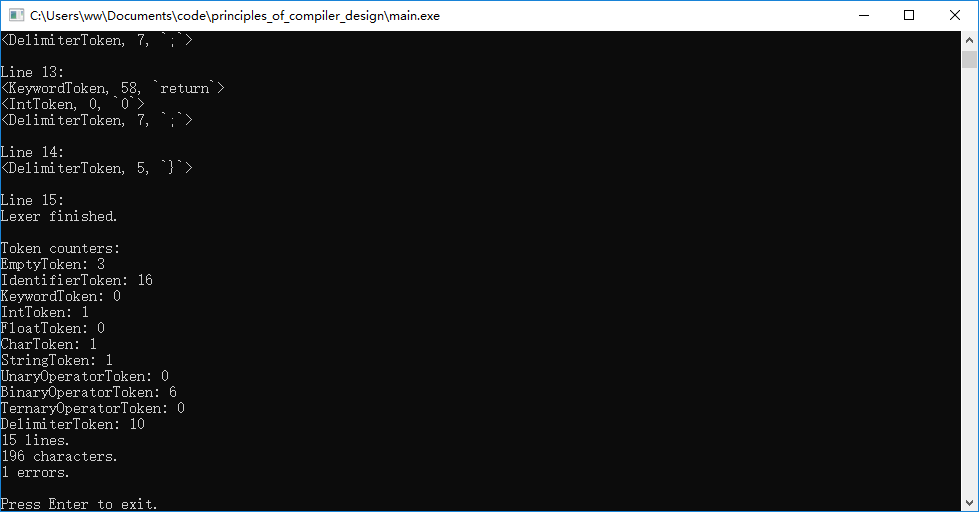
\includegraphics[width=\textwidth]{illegal_2}
\begin{lstlisting}
Line 1
<EmptyToken, 1, `include <iostream`>

Line 2:
<EmptyToken, 1, `include <string`>

Line 3:

Line 4:

Line 5:

Line 6:
<EmptyToken, 1, `*
    错误处理测试样例-转义字符
*`>

Line 7:

Line 8:
<KeywordToken, 40, `int`>
<IdentifierToken, 0, `main`>
<DelimiterToken, 0, `(`>
<KeywordToken, 40, `int`>
<IdentifierToken, 1, `argc`>
<DelimiterToken, 6, `,`>
<KeywordToken, 12, `char`>
<KeywordToken, 18, `const`>
<BinaryOperatorToken, 9, `*`>
<IdentifierToken, 2, `argv`>
<DelimiterToken, 2, `[`>
<DelimiterToken, 3, `]`>
<DelimiterToken, 1, `)`>

Line 9:
<DelimiterToken, 4, `{`>

Line 10:
<IdentifierToken, 3, `std`>
<BinaryOperatorToken, 12, `::`>
<IdentifierToken, 4, `string`>
<IdentifierToken, 5, `s`>
<BinaryOperatorToken, 14, `=`>
<StringToken, `string value\n`>
<DelimiterToken, 7, `;`>

Line 11:
<KeywordToken, 12, `char`>
<IdentifierToken, 6, `c`>
<BinaryOperatorToken, 14, `=`>
<ERROR at (11, 16): missing `'` ? Jump to the next line.>
<CharToken, \, `\'`>

Line 12:
<IdentifierToken, 3, `std`>
<BinaryOperatorToken, 12, `::`>
<IdentifierToken, 7, `cout`>
<BinaryOperatorToken, 5, `<<`>
<IdentifierToken, 5, `s`>
<DelimiterToken, 7, `;`>

Line 13:
<KeywordToken, 58, `return`>
<IntToken, 0, `0`>
<DelimiterToken, 7, `;`>

Line 14:
<DelimiterToken, 5, `}`>

Line 15:
Lexer finished.

Token counters:
EmptyToken: 3
IdentifierToken: 16
KeywordToken: 0
IntToken: 1
FloatToken: 0
CharToken: 1
StringToken: 1
UnaryOperatorToken: 0
BinaryOperatorToken: 6
TernaryOperatorToken: 0
DelimiterToken: 10
15 lines.
196 characters.
1 errors.

Press Enter to exit.
\end{lstlisting}
词法分析程序分析出了所有合法的符号,并找到了第$11$行的错误,尝试修正并继续运行至文件末尾,输出错误数$1$。
\section{完成过程中遇到的问题}
\subsection{程序在$g++$下出现的问题}
若使用$g++$(版本号:$8.1.0$)编译本程序,程序有可能重复分析部分代码,但若使用$clang++$(版本号:$7.0.0$)或$Visual Studio 2017$编译
,则不会出现重复分析的问题。此类情况是因为读取源文件使用的$ifstream::read$函数在不同的编译器下行为不同。
\subsection{分析含中文字符的源代码}
在中文$Windows \ 10$环境中,控制台默认使用$GB2312$作为默认编码,若源文件不为$GB2312$编码,则词法分析程序的输出可能会出现乱码。
\section{备注}
\begin{enumerate}
	\item 词法来源:编译器$Clang++$上进行的测试(版本号:$3.9.1$)和互联网($cppreference.com$等);
	\item 假设字符均合法;
	\item 将所有$($, $)$, $[$, $]$, $\{$, $\}$, $,$视为界符,即
	      \begin{enumerate}
		      \item 将$[index]$中的括号视为界符,数字视为常数、标识符或表达式
		      \item 将$(type)$中的括号视为界符,类型视为关键字或标识符
		      \item 将${value1, value2}$中的$,$视为界符
	      \end{enumerate}
	\item 将$static\_cast$, $dynamic\_cast$, $const\_cast$, $reinterpret\_cast$, $new$, $delete$, $typeid$, $noexcept$, $alignof$视为关键字
	\item 暂不考虑运算符$sizeof$, $sizeof...$
	\item 将$=$, $-=$, $+=$, $*=$, $/=$, $\%=$, $\wedge=$, $\&=$, $|=$, $<<$, $>>$, $>>=$, $<<=$, $?$, $:$视为运算符
	\item 暂不考虑``$,$''作为运算符时,先后计算其左值和右值,并返回右值的特性
	\item $IntTokenType$, $FloatTokenType$均为无符号数,故将$(+|-)(digit|float)$中的$+$, $-$视为运算符
\end{enumerate}
\end{document}
